\newpage
\section*{Appendix Table of Contents}
\startcontents[appendix]
\printcontents[appendix]{l}{1}{\setcounter{tocdepth}{2}}
\newpage

\section{More Training Details} \label{app:training_details}

\subsection{OPD Training Details} \label{app:opd_training_details}
For every input prompt during the OPD training, we generate $n=8$ responses. We constrain the maximum prompt length to 1,024 tokens, while the maximum response length is limited to 7,168 tokens. The optimization process spans a single epoch across 8 H800 80G GPUs, utilizing a learning rate of $1 \times 10^{-6}$. We set both the student sampling temperature and the teacher temperature to 1.0, disable KL regularization, and adopt token-mean loss aggregation. Unless otherwise noted, all experiments use the default OPD hyperparameters listed in Table \ref{tab:opd_hyperparameters}.

\begin{table}[htbp]
\centering
\caption{Default hyperparameters for OPD.}
\label{tab:opd_hyperparameters}
\begin{tabular}{lc}
\toprule
\textbf{Item} & \textbf{Value} \\
\midrule
Training temperature & 1.0 \\
Global batch size & 64 \\
Mini batch size & 64 \\
Rollout number & 8 \\
Temperature & 1.0 \\
LogProb top-$K$ & 16 \\
Top-$K$ strategy & Student Top-$K$ \\
Top-$p$ & 1.0 \\
Max prompt length & 1024 \\
Max response length & 7168 \\
Learning rate & 1e-6 \\
Epoch & 1 \\
KL Coefficient & 0.0 \\
\bottomrule
\end{tabular}
\end{table}


\subsection{GRPO Training Details} \label{app:grpo_training_details}
We train DeepSeek-R1-Distill-Llama-8B for one epoch on the dataset 
DeepMath-103K \citep{deepmath}. The main hyperparameters are summarized in Table \ref{tab:grpo_hyperparameters}.

\begin{table}[htbp]
\centering
\caption{Default hyperparameters for GRPO.}
\label{tab:grpo_hyperparameters}
\begin{tabular}{lc}
\toprule
\textbf{Item} & \textbf{Value} \\
\midrule
Training temperature & 1.0 \\
Global batch size & 64 \\
Mini batch size & 64 \\
Rollout number & 8 \\
Temperature & 1.0 \\
Max prompt length & 1024 \\
Max response length & 7168 \\
Learning rate & 1e-6 \\
Epoch & 1 \\
KL Coefficient & 0.0 \\
\bottomrule
\end{tabular}
\end{table}

\section{More Evaluations} \label{app:ood}
To verify whether the performance gains acquired through 1-shot OPD generalize beyond the mathematical domain, we evaluate our models on out-of-distribution benchmarks, including LiveCodeBench for code reasoning and GPQA for scientific reasoning. Specifically, we report the LiveCodeBench and GPQA accuracy for 1-shot OPD models from Table \ref{tab:one_shot_benchmark_performance} in Table \ref{tab:ood_1shot_models}, and the performance of few-shot OPD models from Table \ref{tab:few_shot_performance} in Table \ref{tab:ood_fewshot_models}. The empirical results further validate that our observations remain highly consistent across out-of-distribution tasks. First, 1-shot OPD trained on a single mathematical example successfully transfers reasoning abilities to coding and scientific domain, yielding notable performance gains over the base student model. As shown in Table \ref{tab:ood_1shot_models}, the 1-shot OPD training on single hard problems achieves an average accuracy of $40.5\%$ on LiveCodeBench and $24.2\%$ on GPQA, significantly outperforming the base student model baselines of $32.4\%$ and $19.4\%$, respectively. Second, training on harder problems consistently achieves superior cross domain performance compared to easy problems. According to Table \ref{tab:ood_1shot_models}, the average accuracy of 1-shot OPD on hard problems ($40.5\%$ on LiveCodeBench and $24.2\%$ on GPQA) markedly surpasses that training on easy problems ($37.6\%$ on LiveCodeBench and $22.1\%$ on GPQA). Third, distilling on 8 selected hard examples is sufficient to closely approach the full dataset baseline. As reported in Table \ref{tab:ood_fewshot_models}, it reaches $42.0\%$ on LiveCodeBench and $27.2\%$ on GPQA, nearly matching the full 17K dataset performance of $42.2\%$ on LiveCodeBench and $27.8\%$ on GPQA.

\begin{table}[htbp]
\centering
\caption{\textbf{Out of Distribution Generalization of 1-Shot OPD Models from Table \ref{tab:one_shot_benchmark_performance}.} We report the accuracy on LiveCodeBench (LCB) and GPQA across individual models. The \textbf{Avg} rows denote the average accuracy across the 8 models trained on Easy, Medium, and Hard samples, respectively.}
\label{tab:ood_1shot_models}
\small
\begin{tabular}{lcccccccr}
\toprule
\multicolumn{3}{c}{\textbf{Easy Problems}} & \multicolumn{3}{c}{\textbf{Medium Problems}} & \multicolumn{3}{c}{\textbf{Hard Problems}} \\
\cmidrule(lr){1-3} \cmidrule(lr){4-6} \cmidrule(lr){7-9}
\textbf{Model} & \textbf{LCB} & \textbf{GPQA} & \textbf{Model} & \textbf{LCB} & \textbf{GPQA} & \textbf{Model} & \textbf{LCB} & \textbf{GPQA} \\
\midrule
$\{\pi_{5}\}$ & 37.3 & 21.4 & $\{\pi_{316}\}$ & 39.3 & 22.2 & $\{\pi_{874}\}$ & 40.9 & 24.6 \\
$\{\pi_{20}\}$ & 38.3 & 21.1 & $\{\pi_{487}\}$ & 39.6 & 23.7 & $\{\pi_{890}\}$ & 40.1 & 23.4 \\
$\{\pi_{21}\}$ & 37.1 & 23.5 & $\{\pi_{530}\}$ & 39.4 & 23.0 & $\{\pi_{948}\}$ & 41.8 & 25.9 \\
$\{\pi_{63}\}$ & 38.8 & 21.6 & $\{\pi_{543}\}$ & 38.9 & 22.3 & $\{\pi_{954}\}$ & 40.8 & 23.7 \\
$\{\pi_{84}\}$ & 36.9 & 22.7 & $\{\pi_{661}\}$ & 39.1 & 23.6 & $\{\pi_{961}\}$ & 39.7 & 23.8 \\
$\{\pi_{105}\}$ & 36.8 & 21.5 & $\{\pi_{763}\}$ & 40.0 & 24.8 & $\{\pi_{973}\}$ & 39.3 & 23.1 \\
$\{\pi_{178}\}$ & 38.7 & 23.1 & $\{\pi_{794}\}$ & 39.4 & 22.7 & $\{\pi_{987}\}$ & 40.4 & 24.3 \\
$\{\pi_{192}\}$ & 37.0 & 21.9 & $\{\pi_{820}\}$ & 38.4 & 22.3 & $\{\pi_{997}\}$ & 40.8 & 24.5 \\
\midrule
\textbf{Avg} & \textbf{37.6} & \textbf{22.1} & \textbf{Avg} & \textbf{39.3} & \textbf{23.1} & \textbf{Avg} & \textbf{40.5} & \textbf{24.2} \\
\bottomrule
\end{tabular}

\caption{\textbf{Out of Distribution Generalization of Few-Shot OPD Models from Table \ref{tab:few_shot_performance}.} We report the average accuracy in LiveCodeBench and GPQA.}
\label{tab:ood_fewshot_models}
\small
\begin{tabular}{lccc}
\toprule
\textbf{Model} & \textbf{Size} & \textbf{LiveCodeBench } & \textbf{GPQA} \\
\midrule
Student & \text{N/A} & 32.4 & 19.4 \\
Teacher & \text{N/A} & 42.8 & 28.0 \\
DAPO-Math-17K & 17K & 42.2 & 27.8 \\
\midrule
$\{\pi_{5}, \pi_{20}, \dots, \pi_{192}\}$ & 8 & 40.6 & 23.7 \\
$\{\pi_{316}, \pi_{487}, \dots, \pi_{820}\}$ & 8 & 40.1 & 24.1 \\
Random & 8 & 40.3 & 24.3 \\
\midrule
$\{\pi_{874}, \pi_{890}, \pi_{954}, \pi_{973}\}$ & 4 & 41.4 & 24.8 \\
$\{\pi_{874}, \dots, \pi_{997}\}$ & 8 & 42.0 & 27.2 \\
$\{\pi_{874}, \dots, \pi_{997}, \dots\}$ & 16 & 40.6 & 26.7 \\
$\{\pi_{874}, \dots, \pi_{997}, \dots\}$ & 64 & 41.7 & 27.5 \\
\bottomrule
\end{tabular}
\end{table}

\section{More Experiments}
\subsection{1-shot OPD in Coding Domain} \label{app:coding}
To evaluate whether our findings generalize beyond mathematical reasoning, we extend our empirical investigation to the code generation domain using the LeetCodeDataset v3.0.1 \citep{xia2025leetcodedataset}, comprising 2,641 problems in total. The dataset provides pre-existing difficulty classifications, containing 638 Easy, 1,397 Medium, and 606 Hard problems. Directly utilizing these native difficulty tags, we sample single training prompts from the Easy, Medium, and Hard categories, respectively. We employ DeepSeek-R1-Distill-Qwen-1.5B as the student model and JustRL-DeepSeek-1.5B as the teacher model. For evaluation, we track LiveCodeBench as the in distribution validation set. To monitor out of distribution performance, we average the accuracy across AMC23, AIME24, and AIME25 as Math Accuracy metric. As illustrated in Figure 6, 1-shot OPD trained on code generation tasks yields substantial validation gains across training steps, while the steady convergence of distillation loss shows effective policy alignment between the student and teacher models. Furthermore, consistent with our mathematical domain observations, distilling on hard coding problems achieves superior performance on both in-distribution and out-of-distribution metrics compared to easy or medium problems.

\begin{figure}[htbp]
    \centering
    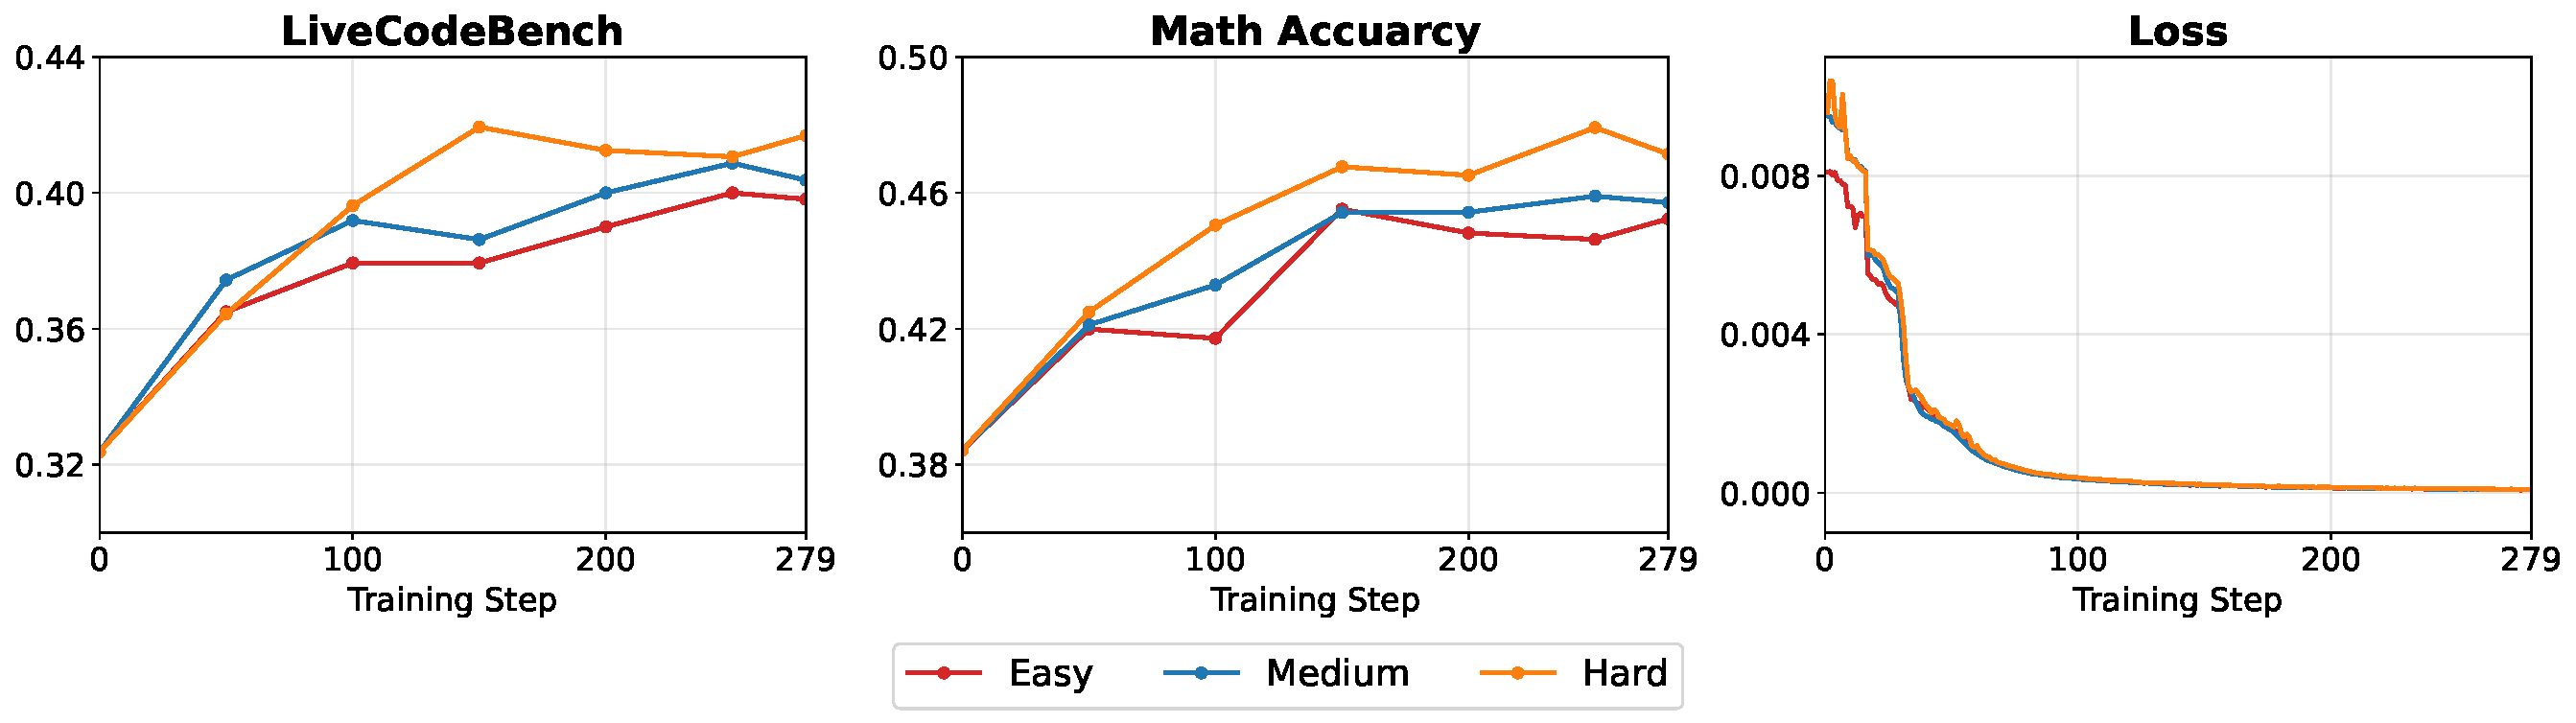
\includegraphics[width=\textwidth]{./images/code.pdf}
    \caption{\textbf{Training dynamics and validation trajectories of 1-shot OPD in the coding domain.} We report the in-distribution validation accuracy on LiveCodeBench, the out of distribution Math Accuracy (computed as the average accuracy across AMC23, AIME24, and AIME25), and the distillation loss over training steps. }
    \label{fig:code_training}
\end{figure}

To further evaluate whether our difficulty-driven data selection strategy remains effective in the coding domain, we conduct experiments scaling training prompts from the LeetCodeDataset. Specifically, we randomly sample 8 hard problems to construct our Hard dataset. For comparison, we establish a Full-Set baseline using the entire LeetCodeDataset of 2,641 problems, as well as a Random baseline trained on 8 randomly sampled problems across all difficulty levels. As reported in Table \ref{tab:coding_data_selection}, our difficulty-driven data selection demonstrates efficiency in the coding domain. Training on only 8 selected hard coding problems yields an average accuracy of $47.1\%$, significantly outperforming the Random baseline ($45.1\%$) and nearly recovering the entire performance ceiling of the Full-Set baseline ($47.3\%$). These results indicate that our data selection strategy generalizes robustly to code generation.

\begin{table}[htbp]
\centering
\caption{\textbf{Data Selection Efficacy in the Coding Domain.} We report benchmark performance across six mathematical reasoning benchmarks alongside LiveCodeBench and GPQA. We evaluate the student model (DeepSeek-R1-Distill-Qwen-1.5B) distilled on LeetCodeDataset training prompts under different selection strategies.}
\label{tab:coding_data_selection}
\small
\resizebox{\textwidth}{!}{
\begin{tabular}{lccccccccccc}
\toprule
\textbf{Model} & \textbf{Size} & \textbf{AIME24} & \textbf{AIME25} & \textbf{AMC23} & \textbf{MATH500} & \textbf{Olympiad} & \textbf{Minerva} & \textbf{LiveCodeBench} & \textbf{GPQA} & \textbf{Avg} \\
\midrule
Student & \text{N/A} & 31.7 & 23.0 & 60.7 & 82.6 & 34.1 & 22.4 & 32.4 & 19.4 & 38.3 \\
Teacher & \text{N/A} & 55.8 & 35.8 & 83.4 & 87.4 & 43.4 & 29.8 & 42.8 & 28.0 & 50.8 \\
\midrule
Full-Set & 2641 & 44.4 & 32.1 & 78.7 & 86.3 & 40.8 & 27.0 & 42.7 & 26.4 & 47.3 \\
\midrule
Random & 8 & 41.2 & 29.0 & 72.0 & 86.1 & 39.3 & 26.1 & 41.6 & 25.6 & 45.1 \\
Hard & 8 & \textbf{43.7} & \textbf{31.8} & \textbf{77.2} & \textbf{87.7} & \textbf{39.9} & \textbf{27.0} & \textbf{42.8} & \textbf{26.3} & \textbf{47.1} \\
\bottomrule
\end{tabular}}
\end{table}

\subsection{1-shot OPD over Extended Training}

We further investigate whether 1-shot OPD suffers from overfitting. To do so, we perform a prolonged training experiment by extending the optimization duration to 2,000 steps for 1-shot OPD training on $\{\pi_{105}\}$, $\{\pi_{794}\}$, and $\{\pi_{973}\}$, respectively. As shown in Figure \ref{fig:long_training}, we observe that the validation accuracy across all three models rises steadily during the first 300 steps and subsequently remains remarkably stable up to 2,000 steps, showing no signs of performance decay or catastrophic policy collapse. This behavior is fundamentally different from SFT and RL in single-example settings \citep{wang2026reinforcement}, which often suffer from severe overfitting or policy degradation under extended optimization. One potential reason is that the sequence-level KL divergence between the teacher and student models naturally decreases as training progresses, leading to loss convergence and preventing policy collapse even under prolonged training.

\begin{figure}[htbp]
    \centering
    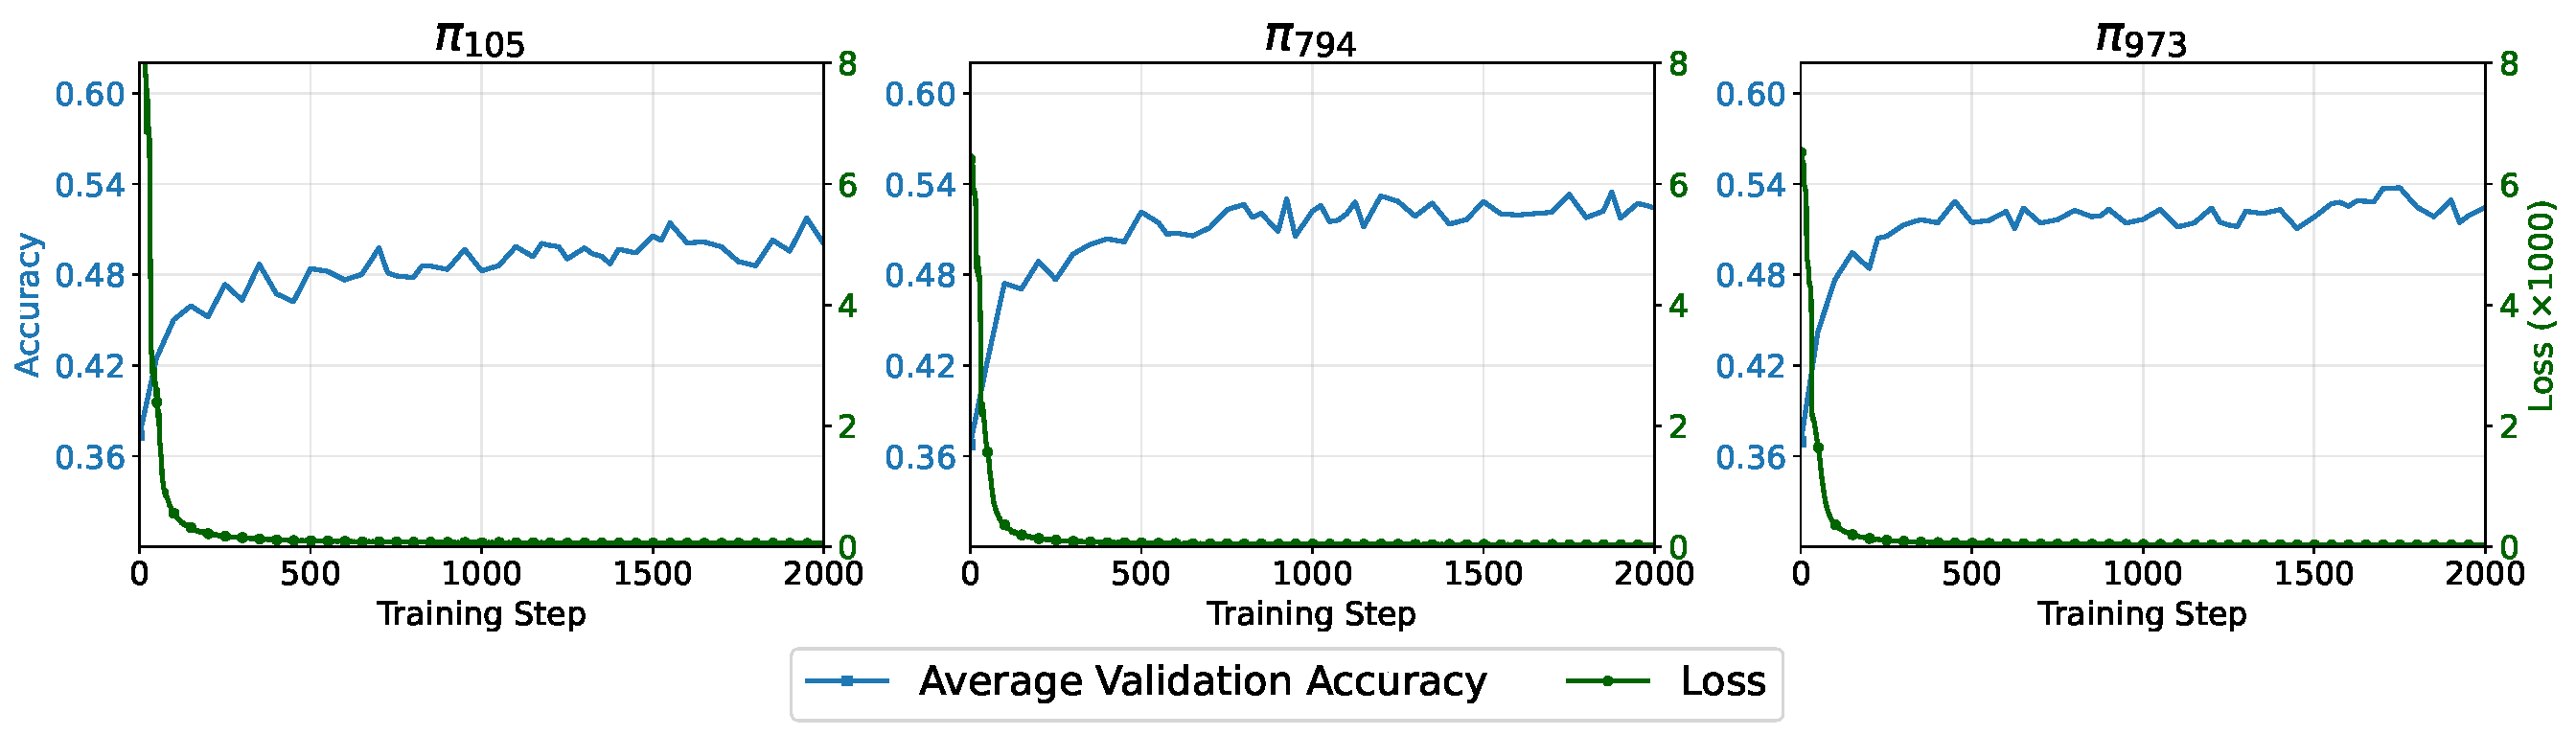
\includegraphics[width=\textwidth]{./images/long.pdf}
    \caption{\textbf{Validation Accuracy over Extended Training in 1-Shot OPD.} We plot the validation trajectories over 2,000 steps for 1-shot OPD models trained on three representative examples of varying difficulty levels: $\{\pi_{105}\}$ (Easy, left), $\{\pi_{794}\}$ (Medium, middle), and $\{\pi_{973}\}$ (Hard, right). Despite extended training, the validation performance across all models remains exceptionally stable without policy collapse.}
    \label{fig:long_training}
\end{figure}

\subsection{1-shot OPD under Different CoT Lengths} \label{app:kl_position}

\begin{wrapfigure}{r}{0.4\linewidth}
    \vspace{-1em}
    \centering
    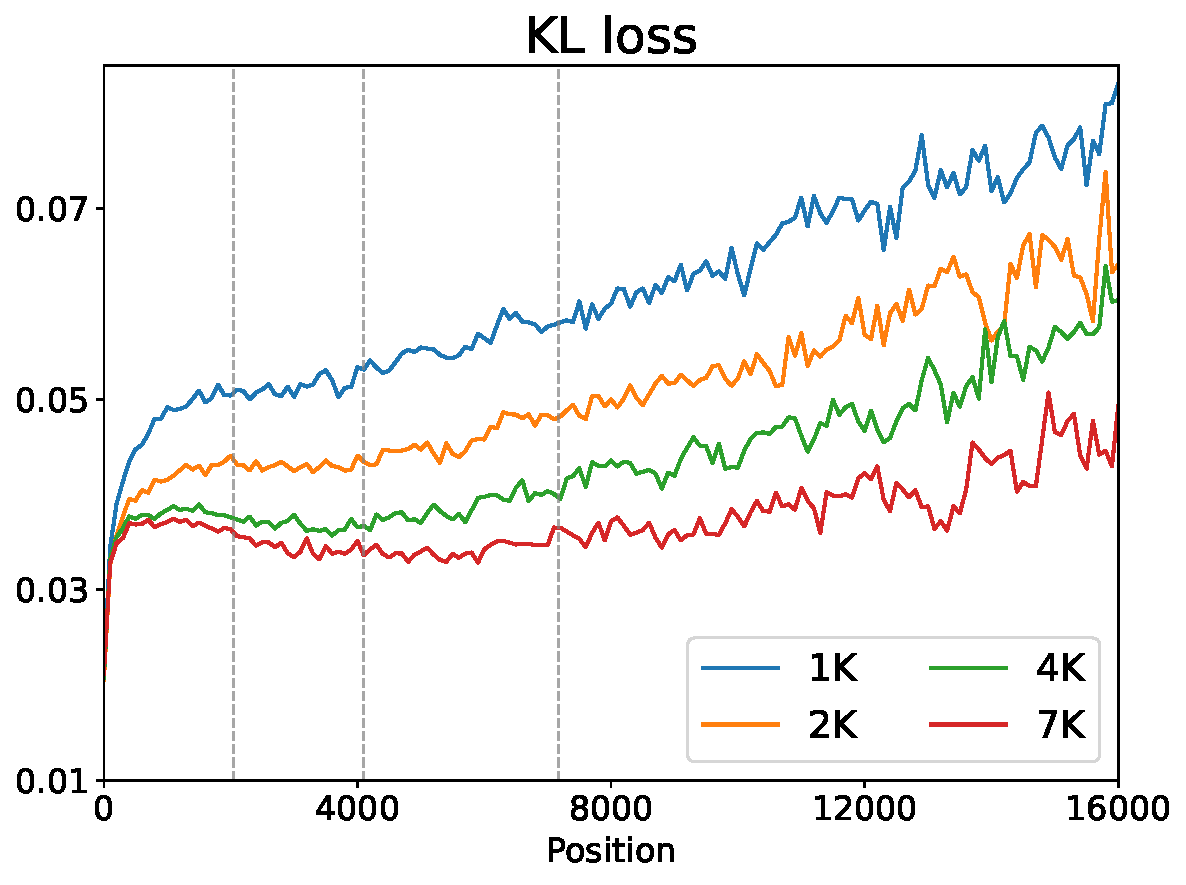
\includegraphics[width=\linewidth]{./images/kl_position.pdf}
    \caption{\textbf{Token-level KL Loss over Generation Position.} For visual clarity, we partition the token positions into non-overlapping intervals of 100 tokens and plot the binned average KL loss over positions.}
    \label{fig:longer_cot_kl_loss}
    \vspace{-1em}
\end{wrapfigure}


 We further compare student models distilled on the hard problem $\{\pi_{954}\}$ under maximum rollout length constraints of 1024, 2048, 4096, and 7168 tokens (referred to as the 1K, 2K, 4K, and 7K models, respectively). For evaluation, we generate 16 rollout completions per problem across the 100 held-out problems. At each generation step, we compute the per-token KL divergence between the distilled student and the teacher policies and plot the average KL loss over positions in Figure \ref{fig:longer_cot_kl_loss}.  The empirical results in Figure \ref{fig:longer_cot_kl_loss} reveal that the 7K model consistently maintains a lower KL divergence across the entire generation horizon compared to the 1K, 2K and 4K models. Crucially, while the alignment of the 4K model is nearly identical to that of the 7K model within the $0$ to $4,000$ token range, the KL gap between them widens significantly as the generation horizon expands beyond $4,000$ tokens. This divergence demonstrates that training on longer CoT sequences directly enhances the model's longer-horizon reasoning capabilities, enabling it to sustain policy alignment with the teacher over extended context lengths.


\subsection{1-shot OPD under Different Temperature} 
We conduct an auxiliary experiment by varying the student rollout temperature $T$ in $\{0.6, 0.8, 1.0, 1.1\}$ during 1-shot OPD. This experiment is specifically designed around one easy problem $\pi_{178}$. By adjusting the sampling temperature of the rollout, we artificially inflate the token-level entropy of the student model's rollouts without altering the inherent difficulty of the training example itself. As illustrated in Figure \ref{fig:temperature}, while higher temperatures markedly elevate the average token entropy throughout training, the corresponding validation accuracy almost keep unchanged across all temperature settings. This empirical result demonstrates that increasing token entropy does not translate to validation gains.

\begin{figure}[h]
    \centering
    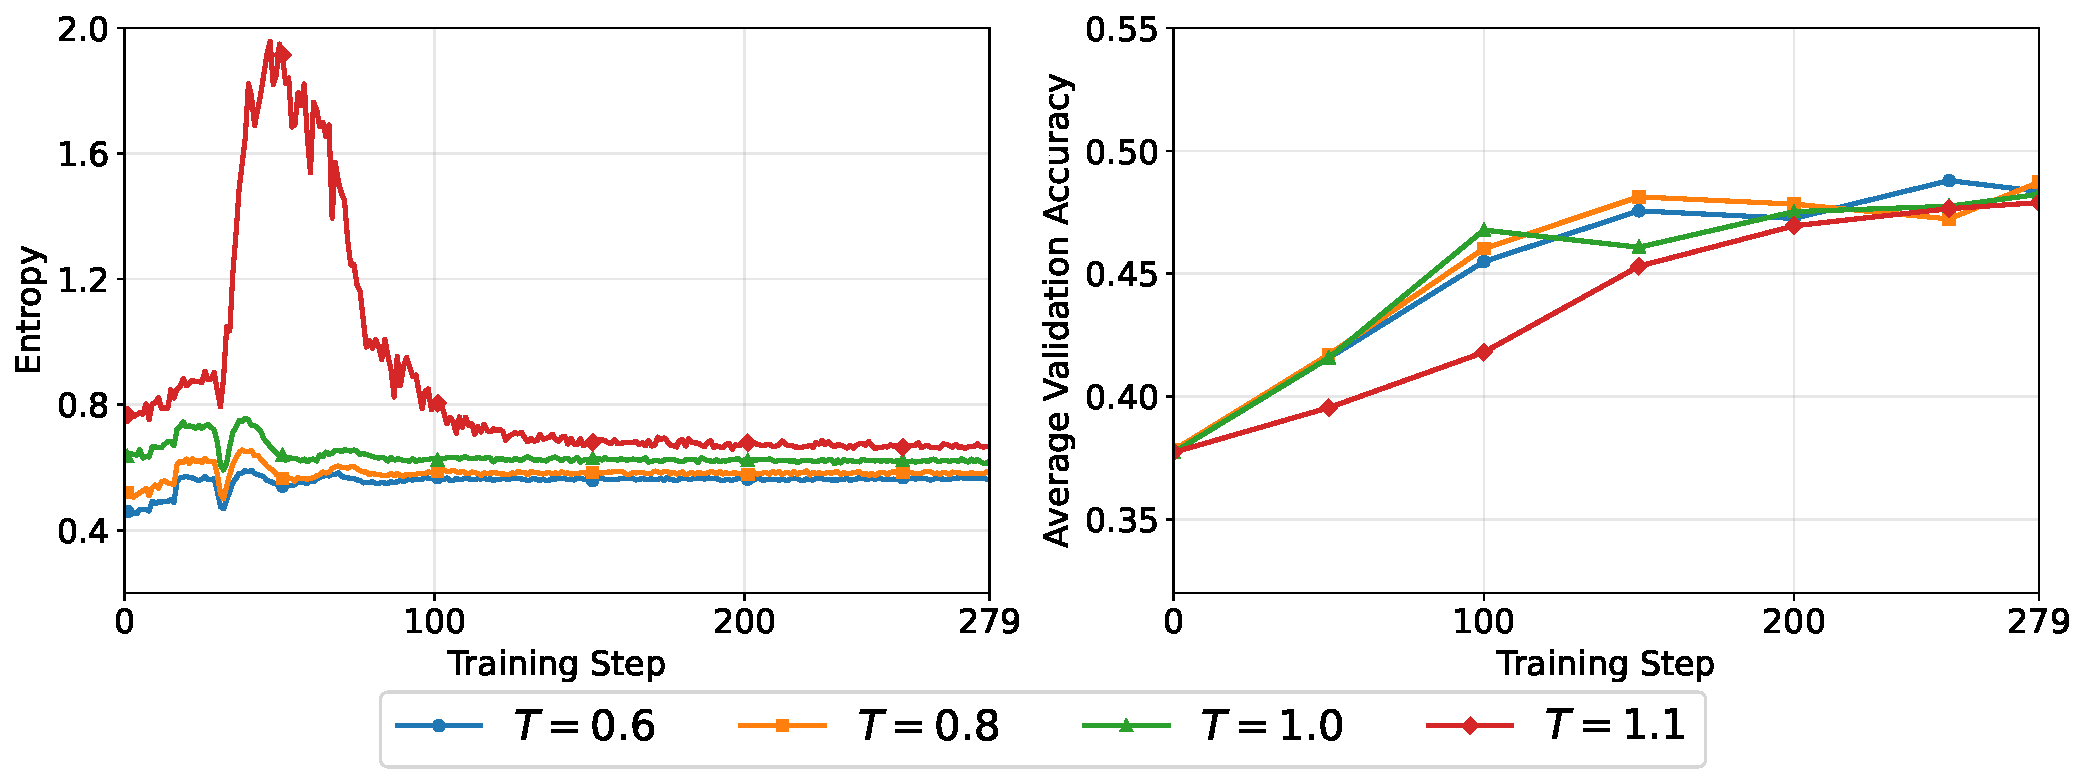
\includegraphics[width=\linewidth]{./images/temperature.pdf}
    \caption{\textbf{Study on student rollout temperature $T$ for the easy example $\pi_{178}$ during 1-shot OPD.} The left subfigure monitors the average per-token entropy of the student's rollouts across training steps under different sampling temperatures $T \in \{0.6, 0.8, 1.0, 1.1\}$. The right subfigure tracks the corresponding Average Validation Accuracy (computed over AMC 2023, AIME 2024, and AIME 2025).}
    \label{fig:temperature}
\end{figure}


\section{Robustness of Data Selection to Random Seeds} \label{app:random_seed}

To evaluate the stability and robustness of our data selection method against sampling randomness, we extend the setup in Section \ref{subsubsec:few_shot_scaling} by introducing two additional independent random seeds, totaling three independent seeds. Specifically, for each seed, we sample a distinct subset of 8 Hard problems (Hard 8) as well as 8 Random problems (Random 8) from the training pool, where the first seed corresponds to that reported in the main text. All models are evaluated using the student model (DeepSeek-R1-Distill-Qwen-1.5B) and the teacher model (JustRL-DeepSeek-1.5B) across eight benchmarks, comprising six mathematical reasoning tasks alongside LiveCodeBench and GPQA. As reported in Table \ref{tab:seed_robustness}, the performance of our data selection consistently outperforms the random selection across all seeds.



\begin{table}[htbp]
\centering
\caption{\textbf{Robustness of Data Selection Across Different Random Seeds.} We report benchmark accuracies across eight evaluation benchmarks alongside their average (Avg) for different data selection under three independent random sampling seeds. Group 1 represents the default seed used in the main text, while Group 2 and Group 3 represent additional independent random seeds.}
\label{tab:seed_robustness}
\small
\resizebox{\textwidth}{!}{
\begin{tabular}{lcccccccccc}
\toprule
\textbf{Model} & \textbf{AIME24} & \textbf{AIME25} & \textbf{AMC23} & \textbf{MATH500} & \textbf{Olympiad} & \textbf{Minerva} & \textbf{LiveCodeBench} & \textbf{GPQA} & \textbf{Avg} \\
\midrule
\multicolumn{10}{l}{\textit{Random Data Selection}} \\
Seed 1 & 48.1 & 33.8 & 76.2 & 86.3 & 41.9 & 26.4 & 40.3 & 24.3 & 47.2 \\
Seed 2 & 46.7 & 35.0 & 76.1 & 87.0 & 41.6 & 26.1 & 39.9 & 21.9 & 46.8 \\
Seed 3 & 46.2 & 33.8 & 77.0 & 86.4 & 42.4 & 26.2 & 40.1 & 24.9 & 47.1 \\
\midrule
\multicolumn{10}{l}{\textit{Our Data Selection}} \\
Seed 1 & 51.7 & 34.2 & 79.2 & 87.2 & 42.7 & 26.4 & 42.0 & 27.2 & \textbf{48.8} \\
Seed 2 & 50.3 & 34.3 & 78.8 & 87.1 & 42.0 & 28.1 & 41.7 & 27.6 & \textbf{48.7} \\
Seed 3 & 51.3 & 34.9 & 79.3 & 87.5 & 42.3 & 27.8 & 42.2 & 27.8 & \textbf{49.1} \\
\bottomrule
\end{tabular}}
\end{table}

% \subsection{Distillation Benefits from Longer CoTs} 

% We explore whether the benefit of longer CoT generated by hard problem arises simply from training on a larger volume of tokens, or if these longer CoTs are inherently better in quality. To study this, we train on the DAPO-Math-17K dataset but implement a length-based filtering strategy during training. Specifically, in each batch, we rank the generated responses by length and update the model using only the top $10\%$ or top $30\%$ longest responses, discarding all other data. The core objective of this design is to drastically reduce the total number of training tokens processed during distillation while preserving only the longest reasoning trajectories. If the advantage of long CoT is purely a matter of token volume, this severe reduction in token cloud lead to a massive drop in validation performance.

% \begin{table}[h]
% \centering
% \caption{\textbf{OPD Performance under Length-Based Response Filtering.} We report benchmark accuracies across different filtering ratios of the \texttt{DAPO-Math-17K} dataset. The average accuracy (Avg) is computed over AIME24, AIME25, and AMC23.}
% \label{tab:length_filtering_performance}
% \small
% \begin{tabular}{lccccc}
% \toprule
% \textbf{Configuration} & \textbf{Data Ratio} & \textbf{AIME24} & \textbf{AIME25} & \textbf{AMC23} & \textbf{Avg } \\
% \midrule
% Full-Set Baseline & $100\%$ & 51.9 & 34.0 & 78.9 & 54.9 \\
% \midrule
% Top-$30\%$ Longest & $30\%$ & 50.6 & 34.4 & 79.1 & 54.7 \\
% Top-$10\%$ Longest & $10\%$ & 49.3 & 34.2 & 78.7 & 54.1 \\
% \bottomrule
% \end{tabular}
% \end{table}

% Surprisingly, we observe that optimizing the policy using only the top $10\%$ longest responses within each batch, which heavily reduces the number of tokens used for gradient updates, yields an average score of $54.1\%$, within $0.8\%$ of the baseline trained on $100\%$ of the dataset ($54.9\%$). Restricting updates to the top $30\%$ longest responses narrows this difference to just $0.2\%$. These results suggest that the reasoning steps in long CoT responses is high-quality for OPD.

\section{Limitations}

A key limitation of our work is that our difficulty-driven data selection is a simple empirical choice rather than a mathematically optimal one. Finding the theoretically optimal training sets for OPD may be computationally intractable. However, despite not being theoretically optimal, our method is extremely simple to use. It requires zero complex optimization, zero extra training parameters, and can be implemented simply by sorting accuracy of examples. We believe this extreme simplicity and ease of implementation make our findings highly valuable for practical applications.

\section{Discussions}

\paragraph{CoT Length as a Practical Proxy in Verifier-Free Domains.}
In mathematical and coding domains, rule-based verifiers are readily available to compute rollout accuracy for task selection. However, in many general reasoning domains, such verifiers do not exist, making difficulty-based selection impossible. For these domains, our findings suggest a simple and effective alternative: using the length of the CoT as a proxy for data selection. As demonstrated in Section \ref{sec:selection}, CoT length is the key driver of policy alignment. Distilling on longer CoT sequences not only enables the student model to maintain alignment stability over a long reasoning horizon, but also successfully activates advanced reasoning patterns (e.g. reflection), that may miss in short trajectories. 

\paragraph{Discussion on Hard Problems with Short Response.} 
A natural question arises regarding potential edge cases in our difficulty-driven selection strategy: what if a problem is categorized as hard due to low model accuracy, yet yields relatively short CoT reasoning responses? We term such instances pseudo-hard problems. These cases often stem from subtle trick questions, common calculation traps, or counterintuitive prompts where models frequently make premature errors without engaging in multi-step exploration. Because these prompts fail to elicit essential reasoning behaviors such as self-reflection, error correction, or backtracking, distilling on them may not yield superior performance gains. Nevertheless, our empirical observations indicate that such pseudo-hard examples are exceptionally rare in practice, as problem difficulty and generated response length exhibit a strong positive correlation. Consequently, while difficulty serves as a robust proxy for selection, incorporating response length as a secondary filtering metric could further refine data selection in edge scenarios.

\paragraph{The Limits of Scaling Rollout Horizon and the Exposure Bias Trade-off.}
A natural question is whether continuously increasing the maximum response length will always yield better policy alignment. We argue that there exists a empirical trade-off: while longer trajectories contain richer reasoning patterns, excessively long on-policy rollouts suffer from severe exposure bias. Because OPD optimizes the student policy against its own dynamically sampled trajectories, any reasoning errors made by the student model will compound over a long horizon. This compounding error drifts the student into out-of-distribution states, which significantly degrades the quality of the teacher's policy supervision. The maximum rollout length in our experiment is chosen as 7,168 following the empirical choice in \cite{li2026rethinking}. To train on even longer CoT sequences without policy decay, we think designing the appropriate training algorithm (e.g. Prune-OPD \citep{yang2026prune}) is necessary.

\section{Example Details} \label{app:sample_details}

\subsection{Accuracy of Sampled Examples}
To classify the difficulty of tasks in our example pool and select representative problems, we evaluate the baseline performance of both the student and teacher models. Specifically, we run 16 independent rollouts per problem for the student model (DeepSeek-R1-Distill-Qwen-1.5B) and the teacher model (JustRL-DeepSeek-1.5B), respectively. For each problem $i$, let $S_i$ and $T_i$ denote the rollout accuracies of the student and teacher models. We then compute the average accuracy as $A_i = (S_i + T_i)/2$ to represent the task difficulty.

Based on this metric, we rank all training examples and group them into three categories: (1) Easy ($A_i > 0.9$), (2) Medium ($0.1 \le A_i \le 0.9$), and (3) Hard ($A_i < 0.1$). Table \ref{tab:opd_accuracies} reports the detailed rollout accuracies of both models on the representative training problems selected in our experiments.

\begin{table}[htbp]
\centering
\caption{\textbf{Accuracies of Sampled Problems.} We report the rollout accuracies of both the student and teacher models across 16 rollouts per problem during our data preparation phase.}
\label{tab:opd_accuracies}
\small
\begin{tabular}{lcc|lcc|lcc}
\toprule
\multicolumn{3}{c}{\textbf{Easy Problems}} & \multicolumn{3}{c}{\textbf{Medium Problems}} & \multicolumn{3}{c}{\textbf{Hard Problems}} \\
\cmidrule(lr){1-3} \cmidrule(lr){4-6} \cmidrule(lr){7-9}
\textbf{ID} & \textbf{Student} & \textbf{Teacher} & \textbf{ID} & \textbf{Student} & \textbf{Teacher} & \textbf{ID} & \textbf{Student} & \textbf{Teacher} \\
\midrule
$\pi_{5}$  & 100.0 & 100.0 & $\pi_{316}$ & 68.8 & 100.0 & $\pi_{874}$ & 0.0 & 6.3  \\
$\pi_{20}$  & 100.0 & 100.0 & $\pi_{487}$ & 37.5 & 100.0 & $\pi_{890}$ & 0.0 & 0.0  \\
$\pi_{21}$  & 100.0 & 100.0 & $\pi_{530}$ & 25.0 & 100.0 & $\pi_{948}$ & 0.0 & 0.0  \\
$\pi_{63}$  & 93.8  & 100.0 & $\pi_{543}$ & 50.0 & 75.0  & $\pi_{954}$ & 0.0 & 0.0  \\
$\pi_{84}$  & 93.8  & 100.0 & $\pi_{661}$ & 25.0 & 68.8  & $\pi_{961}$ & 0.0 & 0.0  \\
$\pi_{105}$ & 87.5  & 100.0  & $\pi_{763}$ & 6.3  & 37.5  & $\pi_{973}$ & 0.0 & 0.0  \\
$\pi_{178}$ & 87.5  & 100.0 & $\pi_{794}$ & 0.0  & 37.5  & $\pi_{987}$ & 0.0 & 0.0  \\
$\pi_{192}$ & 87.5  & 100.0   & $\pi_{820}$ & 6.3  & 18.8  & $\pi_{997}$ & 0.0 & 0.0  \\
\bottomrule
\end{tabular}
\end{table}

\subsection{Content of Sampled Examples}

\begin{table}[htbp]
\centering
\caption{\textbf{Details of example} $\pi_{5}$.}
\begin{tabular}{p{0.95\textwidth}}
\toprule
\textbf{Prompt:} \\
\midrule
\footnotesize
\begin{lstlisting}[breaklines=true, basicstyle=\ttfamily, aboveskip=-1.0em, belowskip=0pt, breakindent=0pt]
Let $a$ and $b$ be positive real numbers.  Find the minimum value of
\[a^2 + b^2 + \frac{1}{(a + b)^2}.\]The answer is in the form k\sqrt{m}+n,. Please provide the value of k + m + n. Please reason step by step, and put your final answer within \boxed{{}}.
\end{lstlisting} \\
\midrule
\textbf{Ground truth:} $3$. \\
\bottomrule
\end{tabular}
\end{table}


\begin{table}[htbp]
\centering
\caption{\textbf{Details of example} $\pi_{20}$.}
\begin{tabular}{p{0.95\textwidth}}
\toprule
\textbf{Prompt:} \\
\midrule
\footnotesize
\begin{lstlisting}[breaklines=true, basicstyle=\ttfamily, aboveskip=-1.0em, belowskip=0pt, breakindent=0pt]
In trapezoid $ABCD$ the lengths of the bases $AB$ and $CD$ are 8 and 17 respectively. The legs of the trapezoid are extended beyond $A$ and $B$ to meet at point $E$. What is the ratio of the area of triangle $EAB$ to the area of trapezoid $ABCD$? Express your answer as a common fraction.The answer is in the form rac{m}{n}, where gcd(m, n) = 1. Please provide the value of m + n. Please reason step by step, and put your final answer within \boxed{{}}.
\end{lstlisting} \\
\midrule
\textbf{Ground truth:} $289$. \\
\bottomrule
\end{tabular}
\end{table}


\begin{table}[htbp]
\centering
\caption{\textbf{Details of example} $\pi_{21}$.}
\begin{tabular}{p{0.95\textwidth}}
\toprule
\textbf{Prompt:} \\
\midrule
\footnotesize
\begin{lstlisting}[breaklines=true, basicstyle=\ttfamily, aboveskip=-1.0em, belowskip=0pt, breakindent=0pt]
Lines $l_1^{}$ and $l_2^{}$ both pass through the origin and make first-quadrant angles of $\frac{\pi}{70}$ and $\frac{\pi}{54}$ radians, respectively, with the positive $x$-axis. For any line  $l$, the transformation $R(l)$ produces another line as follows: $l$ is reflected in $l_1$, and the resulting line is reflected in $l_2$. Let $R^{(1)}(l)=R(l)$ and $R^{(n)}(l)=R\left(R^{(n-1)}(l)\right)$. Given that $l$ is the line $y=\frac{19}{92}x$, find the smallest positive integer $m$ for which $R^{(m)}(l)=l$. Please reason step by step, and put your final answer within \boxed{{}}.
\end{lstlisting} \\
\midrule
\textbf{Ground truth:} $945$. \\
\bottomrule
\end{tabular}
\end{table}


\begin{table}[htbp]
\centering
\caption{\textbf{Details of example} $\pi_{63}$.}
\begin{tabular}{p{0.95\textwidth}}
\toprule
\textbf{Prompt:} \\
\midrule
\footnotesize
\begin{lstlisting}[breaklines=true, basicstyle=\ttfamily, aboveskip=-1.0em, belowskip=0pt, breakindent=0pt]
On the party, every boy gave $1$ candy to every girl, and every girl gave $1$ candy to every boy. Then every boy ate $2$ candies, and every girl ate $3$ candies. It is known that $\frac{1}{4}$ of all candies were eaten. Find the greatest possible number of children at the party. Please reason step by step, and put your final answer within \boxed{{}}.
\end{lstlisting} \\
\midrule
\textbf{Ground truth:} $35$. \\
\bottomrule
\end{tabular}
\end{table}


\begin{table}[htbp]
\centering
\caption{\textbf{Details of example} $\pi_{84}$.}
\begin{tabular}{p{0.95\textwidth}}
\toprule
\textbf{Prompt:} \\
\midrule
\footnotesize
\begin{lstlisting}[breaklines=true, basicstyle=\ttfamily, aboveskip=-1.0em, belowskip=0pt, breakindent=0pt]
The prime numbers $a$, $b$, and $c$ satisfy the equation $a + b^2 = 4c^2$. Determine the sum of all possible values of $a + b + c$. Please reason step by step, and put your final answer within \boxed{{}}.
\end{lstlisting} \\
\midrule
\textbf{Ground truth:} $31$. \\
\bottomrule
\end{tabular}
\end{table}


\begin{table}[htbp]
\centering
\caption{\textbf{Details of example} $\pi_{105}$.}
\begin{tabular}{p{0.95\textwidth}}
\toprule
\textbf{Prompt:} \\
\midrule
\footnotesize
\begin{lstlisting}[breaklines=true, basicstyle=\ttfamily, aboveskip=-1.0em, belowskip=0pt, breakindent=0pt]
Compute the smallest positive integer $N$ for which $N \cdot 2^{2024}$ is a multiple of $2024$. Please reason step by step, and put your final answer within \boxed{{}}.
\end{lstlisting} \\
\midrule
\textbf{Ground truth:} $253$. \\
\bottomrule
\end{tabular}
\end{table}


\begin{table}[htbp]
\centering
\caption{\textbf{Details of example} $\pi_{178}$.}
\begin{tabular}{p{0.95\textwidth}}
\toprule
\textbf{Prompt:} \\
\midrule
\footnotesize
\begin{lstlisting}[breaklines=true, basicstyle=\ttfamily, aboveskip=-1.0em, belowskip=0pt, breakindent=0pt]
Determine the number of pairs $(a,b)$ of real numbers such that $10, a, b, ab$ is an arithmetic progression. Please reason step by step, and put your final answer within \boxed{{}}.
\end{lstlisting} \\
\midrule
\textbf{Ground truth:} $2$. \\
\bottomrule
\end{tabular}
\end{table}


\begin{table}[htbp]
\centering
\caption{\textbf{Details of example} $\pi_{192}$.}
\begin{tabular}{p{0.95\textwidth}}
\toprule
\textbf{Prompt:} \\
\midrule
\footnotesize
\begin{lstlisting}[breaklines=true, basicstyle=\ttfamily, aboveskip=-1.0em, belowskip=0pt, breakindent=0pt]
Compute the remainder when $2^{3^5}+ 3^{5^2}+ 5^{2^3}$ is divided by $30$. Please reason step by step, and put your final answer within \boxed{{}}.
\end{lstlisting} \\
\midrule
\textbf{Ground truth:} $6$. \\
\bottomrule
\end{tabular}
\end{table}


\begin{table}[htbp]
\centering
\caption{\textbf{Details of example} $\pi_{316}$.}
\begin{tabular}{p{0.95\textwidth}}
\toprule
\textbf{Prompt:} \\
\midrule
\footnotesize
\begin{lstlisting}[breaklines=true, basicstyle=\ttfamily, aboveskip=-1.0em, belowskip=0pt, breakindent=0pt]
A dartboard consists of three concentric circles with radii 4, 6, and 8. Three darts are thrown at the board, sticking at random locations. Determine the probability that each dart lands in a different region of the dartboard. The probability can be expressed as \( \frac{m}{n} \), where \( m \) and \( n \) are relatively prime positive integers. Calculate \( m + n \). Please reason step by step, and put your final answer within \boxed{{}}.
\end{lstlisting} \\
\midrule
\textbf{Ground truth:} $617$. \\
\bottomrule
\end{tabular}
\end{table}


\begin{table}[htbp]
\centering
\caption{\textbf{Details of example} $\pi_{487}$.}
\begin{tabular}{p{0.95\textwidth}}
\toprule
\textbf{Prompt:} \\
\midrule
\footnotesize
\begin{lstlisting}[breaklines=true, basicstyle=\ttfamily, aboveskip=-1.0em, belowskip=0pt, breakindent=0pt]
In how many ways can the integers from 1 to n be ordered subject to the condition that, except for the first integer on the left, every integer differs by 1 from some integer to the left of it? Please provide the number of ways for $n = 6$. Please reason step by step, and put your final answer within \boxed{{}}.
\end{lstlisting} \\
\midrule
\textbf{Ground truth:} $32$. \\
\bottomrule
\end{tabular}
\end{table}


\begin{table}[htbp]
\centering
\caption{\textbf{Details of example} $\pi_{530}$.}
\begin{tabular}{p{0.95\textwidth}}
\toprule
\textbf{Prompt:} \\
\midrule
\footnotesize
\begin{lstlisting}[breaklines=true, basicstyle=\ttfamily, aboveskip=-1.0em, belowskip=0pt, breakindent=0pt]
Determine the largest integer $N$ for which there exists a $6 \times N$ table $T$ that has the following properties:\n\n- Every column contains the numbers $1, 2, \ldots, 6$ in some ordering.\n- For any two columns $i \ne j$, there exists a row $r$ such that $T(r,i) = T(r,j)$.\n- For any two columns $i \ne j$, there exists a row $s$ such that $T(s,i) \ne T(s,j)$. Please reason step by step, and put your final answer within \boxed{{}}.
\end{lstlisting} \\
\midrule
\textbf{Ground truth:} $120$. \\
\bottomrule
\end{tabular}
\end{table}


\begin{table}[htbp]
\centering
\caption{\textbf{Details of example} $\pi_{543}$.}
\begin{tabular}{p{0.95\textwidth}}
\toprule
\textbf{Prompt:} \\
\midrule
\footnotesize
\begin{lstlisting}[breaklines=true, basicstyle=\ttfamily, aboveskip=-1.0em, belowskip=0pt, breakindent=0pt]
Let f be a polynomial of degree $3$ with integer coefficients such that $f(0) = 3$ and $f(1) = 11$.
If f has exactly $2$ integer roots, how many such polynomials $f$ exist? Please reason step by step, and put your final answer within \boxed{{}}.
\end{lstlisting} \\
\midrule
\textbf{Ground truth:} $0$. \\
\bottomrule
\end{tabular}
\end{table}


\begin{table}[htbp]
\centering
\caption{\textbf{Details of example} $\pi_{661}$.}
\begin{tabular}{p{0.95\textwidth}}
\toprule
\textbf{Prompt:} \\
\midrule
\footnotesize
\begin{lstlisting}[breaklines=true, basicstyle=\ttfamily, aboveskip=-1.0em, belowskip=0pt, breakindent=0pt]
Find the area of the figure on the coordinate plane bounded by the straight lines $x = 0$, $x = 2$, and the graphs of the functions $y = \\sqrt{x^3 + 1}$ and $y = -\\sqrt[3]{x^2 + 2x}$. Please reason step by step, and put your final answer within \\boxed{{}}.
\end{lstlisting} \\
\midrule
\textbf{Ground truth:} $6$. \\
\bottomrule
\end{tabular}
\end{table}


\begin{table}[htbp]
\centering
\caption{\textbf{Details of example} $\pi_{763}$.}
\begin{tabular}{p{0.95\textwidth}}
\toprule
\textbf{Prompt:} \\
\midrule
\footnotesize
\begin{lstlisting}[breaklines=true, basicstyle=\ttfamily, aboveskip=-1.0em, belowskip=0pt, breakindent=0pt]
An organization has $30$ employees, $20$ of whom have a brand A computer while the other $10$ have a brand B computer. For security, the computers can only be connected to each other and only by cables. The cables can only connect a brand A computer to a brand B computer. Employees can communicate with each other if their computers are directly connected by a cable or by relaying messages through a series of connected computers. Initially, no computer is connected to any other. A technician arbitrarily selects one computer of each brand and installs a cable between them, provided there is not already a cable between that pair. The technician stops once every employee can communicate with each other. What is the maximum possible number of cables used? Please reason step by step, and put your final answer within \\boxed{{}}.
\end{lstlisting} \\
\midrule
\textbf{Ground truth:} $191$. \\
\bottomrule
\end{tabular}
\end{table}


\begin{table}[htbp]
\centering
\caption{\textbf{Details of example} $\pi_{794}$.}
\begin{tabular}{p{0.95\textwidth}}
\toprule
\textbf{Prompt:} \\
\midrule
\footnotesize
\begin{lstlisting}[breaklines=true, basicstyle=\ttfamily, aboveskip=-1.0em, belowskip=0pt, breakindent=0pt]
Tanya wrote numbers in the form $n^7 - 1$ for $n = 2, 3, \ldots$ and noticed that for $n = 8$, she obtained a number divisible by $337$. For what minimal $n$ did she get a number divisible by $2022$? Please reason step by step, and put your final answer within \boxed{{}}.
\end{lstlisting} \\
\midrule
\textbf{Ground truth:} $79$. \\
\bottomrule
\end{tabular}
\end{table}


\begin{table}[htbp]
\centering
\caption{\textbf{Details of example} $\pi_{820}$.}
\begin{tabular}{p{0.95\textwidth}}
\toprule
\textbf{Prompt:} \\
\midrule
\footnotesize
\begin{lstlisting}[breaklines=true, basicstyle=\ttfamily, aboveskip=-1.0em, belowskip=0pt, breakindent=0pt]
Vasya has $n$ candies of several types, where $n > 145$. It is known that for any group of at least 145 candies, there is a type of candy which appears exactly 10 times. Find the largest possible value of $n$. Please reason step by step, and put your final answer within \boxed{{}}.
\end{lstlisting} \\
\midrule
\textbf{Ground truth:} $160$. \\
\bottomrule
\end{tabular}
\end{table}


\begin{table}[htbp]
\centering
\caption{\textbf{Details of example} $\pi_{874}$.}
\begin{tabular}{p{0.95\textwidth}}
\toprule
\textbf{Prompt:} \\
\midrule
\footnotesize
\begin{lstlisting}[breaklines=true, basicstyle=\ttfamily, aboveskip=-1.0em, belowskip=0pt, breakindent=0pt]
Find the number of subsets of $\{1,3,5,7,9,11,13,15,17,19\}$ where the elements in the subset add to $49$. Please reason step by step, and put your final answer within \boxed{{}}.
\end{lstlisting} \\
\midrule
\textbf{Ground truth:} $22$. \\
\bottomrule
\end{tabular}
\end{table}


\begin{table}[htbp]
\centering
\caption{\textbf{Details of example} $\pi_{890}$.}
\begin{tabular}{p{0.95\textwidth}}
\toprule
\textbf{Prompt:} \\
\midrule
\footnotesize
\begin{lstlisting}[breaklines=true, basicstyle=\ttfamily, aboveskip=-1.0em, belowskip=0pt, breakindent=0pt]
Let $x_1, x_2, \dots, x_{100}$ be real numbers such that $|x_1| = 63$ and $|x_{n+1}| = |x_n + 1|$ for $n = 1, 2, \dots, 99$. Find the largest possible value of $(-x_1 - x_2 - \cdots - x_{100})$. Please reason step by step, and put your final answer within \boxed{{}}.
\end{lstlisting} \\
\midrule
\textbf{Ground truth:} $2034$. \\
\bottomrule
\end{tabular}
\end{table}


\begin{table}[htbp]
\centering
\caption{\textbf{Details of example} $\pi_{948}$.}
\begin{tabular}{p{0.95\textwidth}}
\toprule
\textbf{Prompt:} \\
\midrule
\footnotesize
\begin{lstlisting}[breaklines=true, basicstyle=\ttfamily, aboveskip=-1.0em, belowskip=0pt, breakindent=0pt]
Two real numbers $x$ and $y$ are chosen at random in the interval (0,1) with respect to the uniform distribution. What is the probability that the closest integer to $x/y$ is even? The original answer is in the form $r + s\pi$, please give the value of $r + s$.  Please reason step by step, and put your final answer within \boxed{{}}.
\end{lstlisting} \\
\midrule
\textbf{Ground truth:} $4$. \\
\bottomrule
\end{tabular}
\end{table}


\begin{table}[htbp]
\centering
\caption{\textbf{Details of example} $\pi_{954}$.}
\begin{tabular}{p{0.95\textwidth}}
\toprule
\textbf{Prompt:} \\
\midrule
\footnotesize
\begin{lstlisting}[breaklines=true, basicstyle=\ttfamily, aboveskip=-1.0em, belowskip=0pt, breakindent=0pt]
Let $f:\{1,2,\dots,2019\}\to\{-1,1\}$ be a function, such that for every $k\in\{1,2,\dots,2019\}$, there exists an $\ell\in\{1,2,\dots,2019\}$ such that $$ \sum_{i\in\mathbb{Z}:(\ell-i)(i-k)\geqslant 0} f(i)\leqslant 0. $$ Determine the maximum possible value of $$ \sum_{i\in\mathbb{Z}:1\leqslant i\leqslant 2019} f(i). $$ Please reason step by step, and put your final answer within \boxed{{}}.
\end{lstlisting} \\
\midrule
\textbf{Ground truth:} $673$. \\
\bottomrule
\end{tabular}
\end{table}


\begin{table}[htbp]
\centering
\caption{\textbf{Details of example} $\pi_{961}$.}
\begin{tabular}{p{0.95\textwidth}}
\toprule
\textbf{Prompt:} \\
\midrule
\footnotesize
\begin{lstlisting}[breaklines=true, basicstyle=\ttfamily, aboveskip=-1.0em, belowskip=0pt, breakindent=0pt]
A herder has forgotten the number of cows she has and does not want to count all of them. She remembers these four facts about the number of cows:\n\n- It has $3$ digits.\n- It is a palindrome.\n- The middle digit is a multiple of $4$.\n- It is divisible by $11$.\n\nWhat is the sum of all possible numbers of cows that the herder has?\n\n$\\textbf{(A) }343 \\ \\textbf{(B) }494 \\ \\textbf{(C) }615 \\ \\textbf{(D) }635 \\ \\textbf{(E) }726$ Please reason step by step, and put your final answer within \\boxed{{}}.
\end{lstlisting} \\
\midrule
\textbf{Ground truth:} $726$. \\
\bottomrule
\end{tabular}
\end{table}


\begin{table}[!t]
\centering
\caption{\textbf{Details of example} $\pi_{973}$.}
\begin{tabular}{p{0.95\textwidth}}
\toprule
\textbf{Prompt:} \\
\midrule
\footnotesize
\begin{lstlisting}[breaklines=true, basicstyle=\ttfamily, aboveskip=-1.0em, belowskip=0pt, breakindent=0pt]
Find all ordered pairs $(a, b)$ of positive integers for which\n$$\n\frac{1}{a}+\frac{1}{b}=\frac{3}{2018} .\n$$\nPlease provide the sum of all integers in the ordered pairs. Please reason step by step, and put your final answer within \boxed{{}}.
\end{lstlisting} \\
\midrule
\textbf{Ground truth:} $1438383$. \\
\bottomrule
\end{tabular}

\caption{\textbf{Details of example} $\pi_{987}$.}
\begin{tabular}{p{0.95\textwidth}}
\toprule
\textbf{Prompt:} \\
\midrule
\footnotesize
\begin{lstlisting}[breaklines=true, basicstyle=\ttfamily, aboveskip=-1.0em, belowskip=0pt, breakindent=0pt]
Find the smallest positive integer $n$ with the following property:  for every sequence of positive integers $a_1,a_2,\ldots , a_n$ with $a_1+a_2+\ldots +a_n=2013$, there exist some (possibly one) consecutive term(s) in the sequence that add up to $70$. Please reason step by step, and put your final answer within \boxed{{}}.
\end{lstlisting} \\
\midrule
\textbf{Ground truth:} $1033$. \\
\bottomrule
\end{tabular}

\caption{\textbf{Details of example} $\pi_{997}$.}
\begin{tabular}{p{0.95\textwidth}}
\toprule
\textbf{Prompt:} \\
\midrule
\footnotesize
\begin{lstlisting}[breaklines=true, basicstyle=\ttfamily, aboveskip=-1.0em, belowskip=0pt, breakindent=0pt]
A quadratic polynomial $f(x)$ is called sparse if its degree is exactly 2 , if it has integer coefficients, and if there exists a nonzero polynomial $g(x)$ with integer coefficients such that $f(x) g(x)$ has degree at most 3 and $f(x) g(x)$ has at most two nonzero coefficients. Find the number of sparse quadratics whose coefficients lie between 0 and 10, inclusive. Please reason step by step, and put your final answer within \boxed{{}}.
\end{lstlisting} \\
\midrule
\textbf{Ground truth:} $228$. \\
\bottomrule
\end{tabular}
\end{table}


